\documentclass{article}

\usepackage{graphicx}
\usepackage{hyperref}
\usepackage{xcolor}
\usepackage[T1]{fontenc}

\title{Students Independent Study 1}
\author{Amangeldi Zhanserik}
\date{05 02 2005}

\begin{document}

\begin{titlepage}
    \centering

    \vspace*{1cm}

    \rule{\textwidth}{1pt}

    \vspace{2\baselineskip}

    {\huge  Cyber Security } \\

    \vspace{1\baselineskip}

    {\huge \textbf{ Lab 3 - Explore Social Engineering Techniques}}

    \vspace{2\baselineskip}

    \rule{\textwidth}{1pt}

    \vspace{1cm}

    \large

    \begin{flushleft}
        \begin{minipage}{.8\textwidth}
            \raggedright
            Fullname: Amangeldi Zhanserik \\
            ID: 22B030301 \\
            E-mail: {\normalsize \url{zha_amangeldi@kbtu.kz}} \\
            Date of submission: 05/02/2025 \\
            Class time: Thursday, 15:00--18:00 \\
        \end{minipage}%
    \end{flushleft}

    \vspace{2cm}

    
\includegraphics[width=.7\textwidth]{logo-kbtu.png}

    \vfill

    School of Information System and Engineering \\
    Kazakh-British Technical University \\
    Academic Year 2024-2025 \\
\end{titlepage}

\section*{Part 1. Explore Social Engineering Techniques}


\subsection*{Step 1: Explore Baiting, Shoulder Surfing, and Pretexting.}

\textbf{Question 1: } What is baiting? Did you click on the USB drive? What happened to the victim's system? \\
\textbf{Answer: } Baiting is a social engineering attack that relies on the curiosity or greed of the victim. In interactive game I clicked to the USB drive and it leading to the installation of malware on the victim's system. \\

\vspace{1\baselineskip}

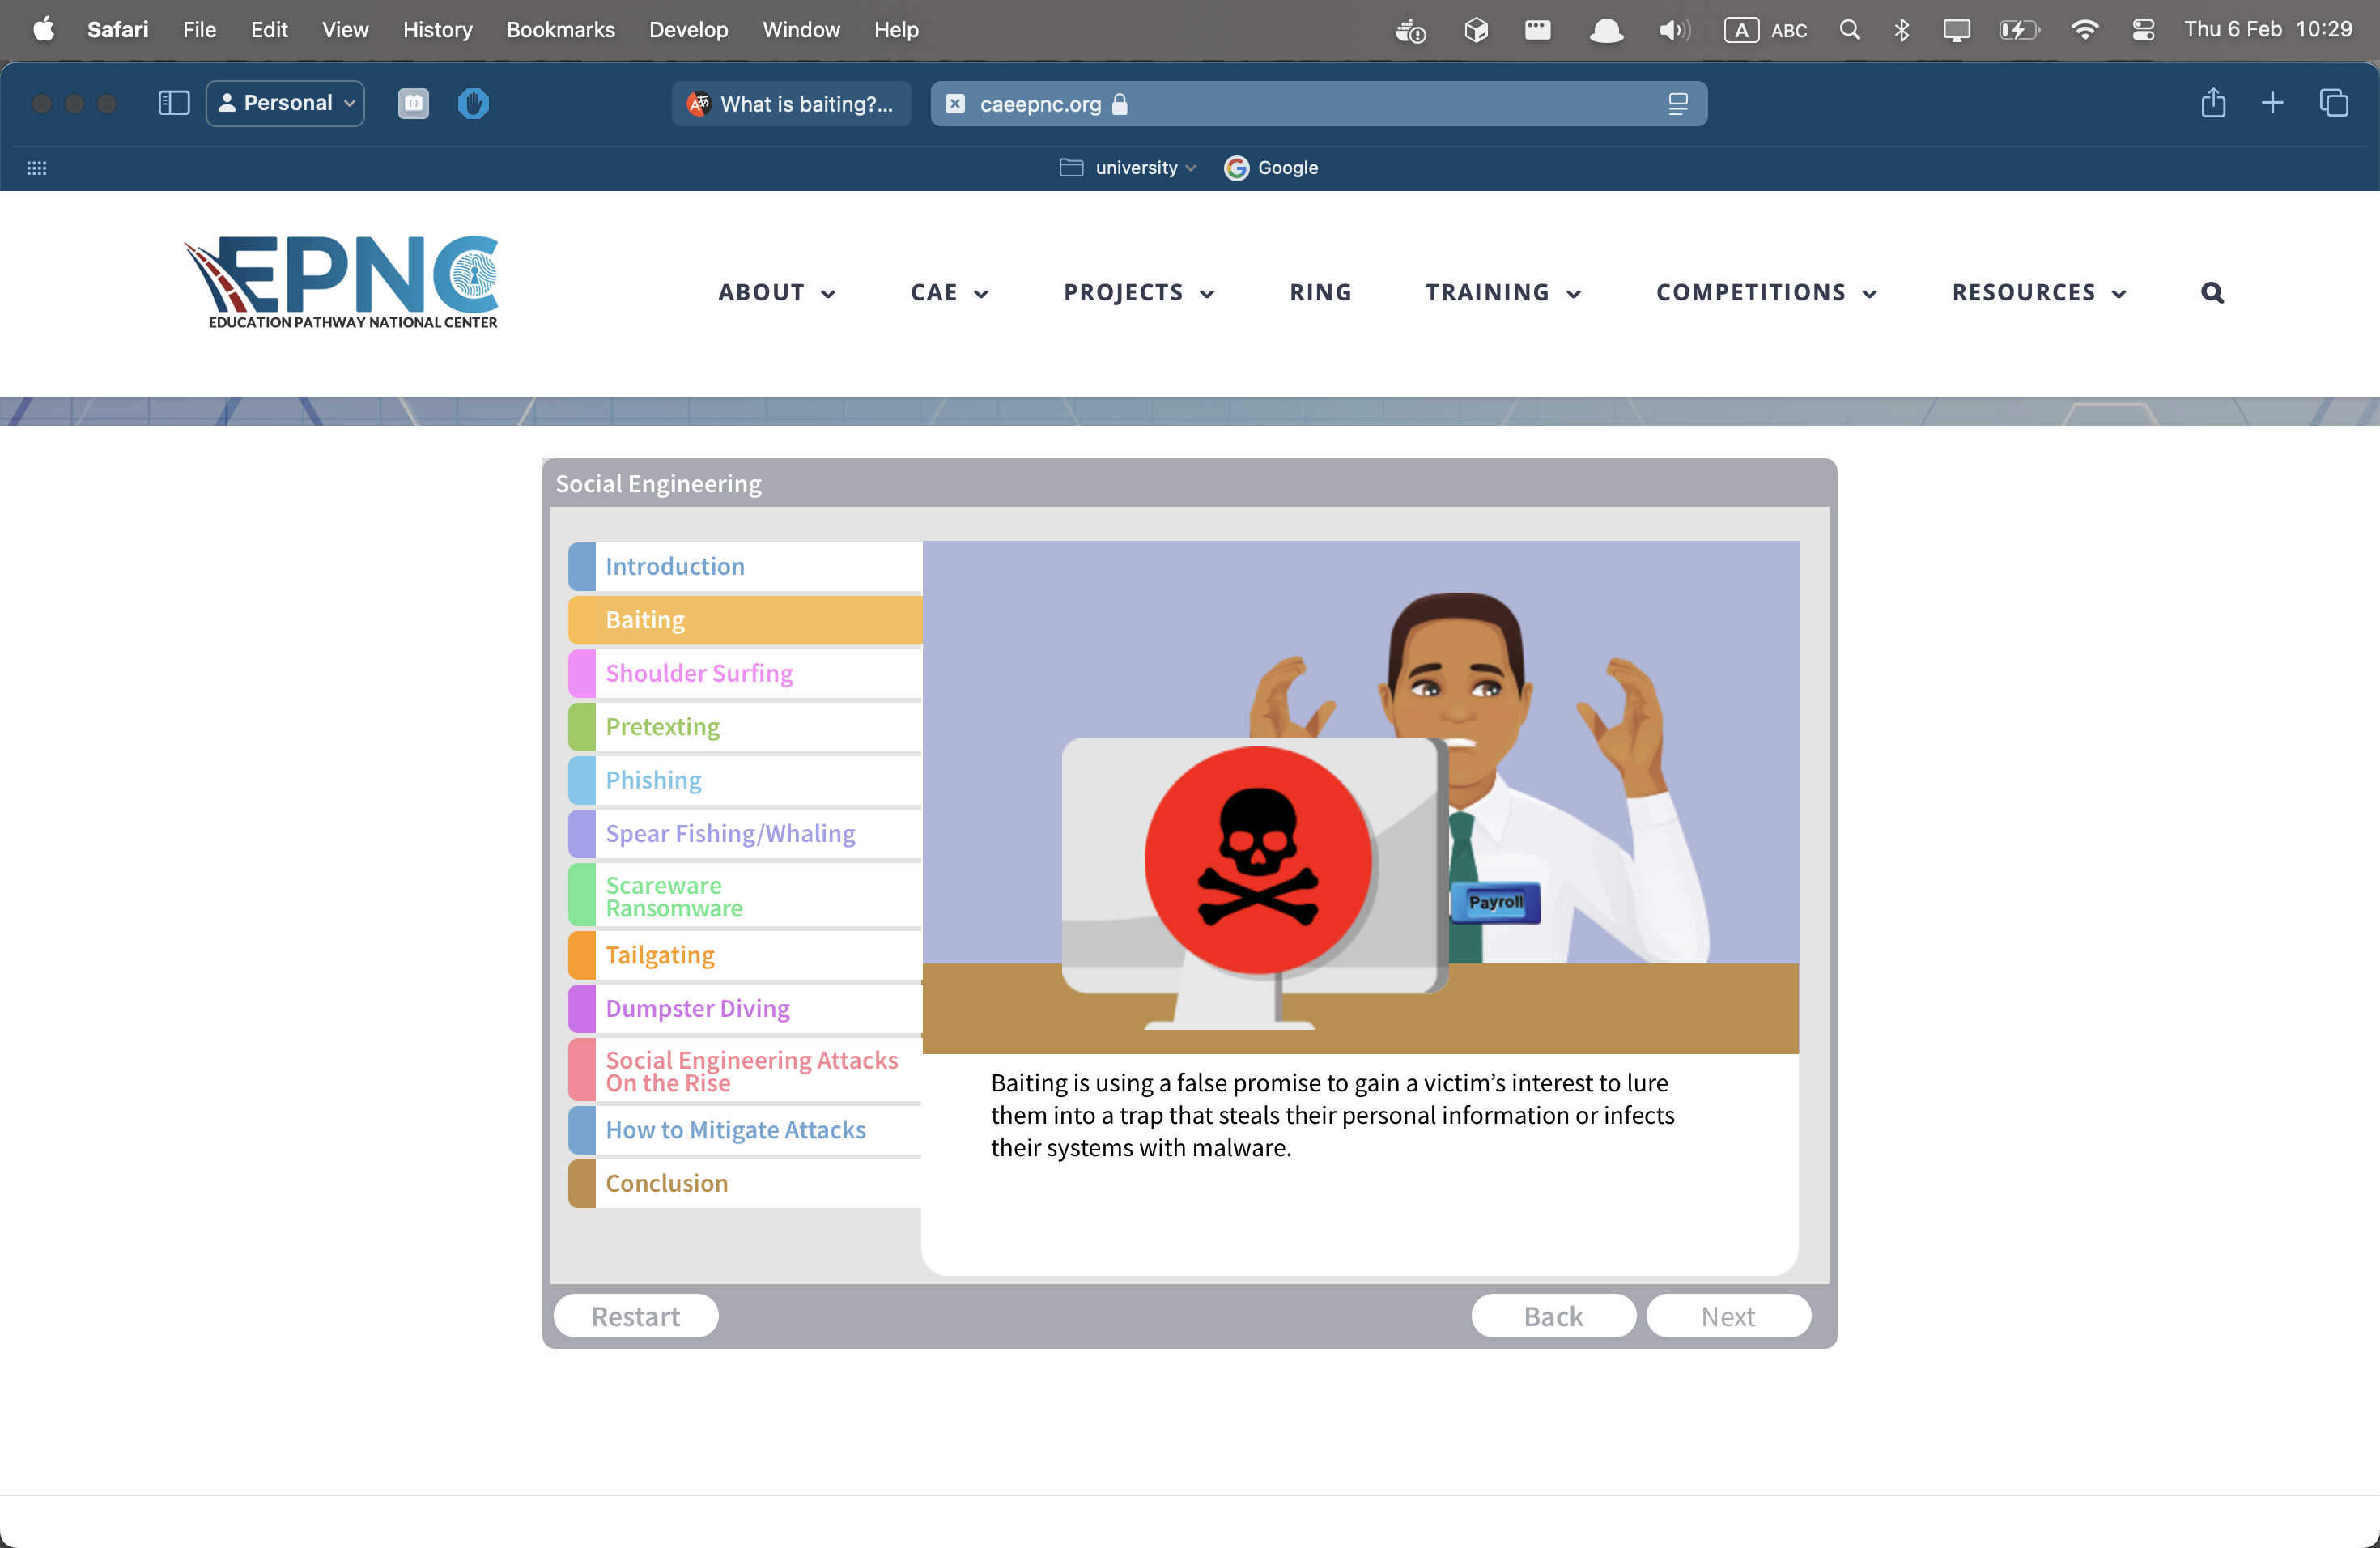
\includegraphics[width=1\textwidth]{1.png}

\newpage

\textbf{Question 2: } What is Shoulder Surfing? What device was used to perform shoulder surfing? What information was gained? \\
\textbf{Answer: } Shoulder surfing is a social engineering attack that involves looking over someone's shoulder to get information. In the interactive game, a smartphone was used to perform shoulder surfing. The information gained was the victim's login and password. \\

\vspace{1\baselineskip}

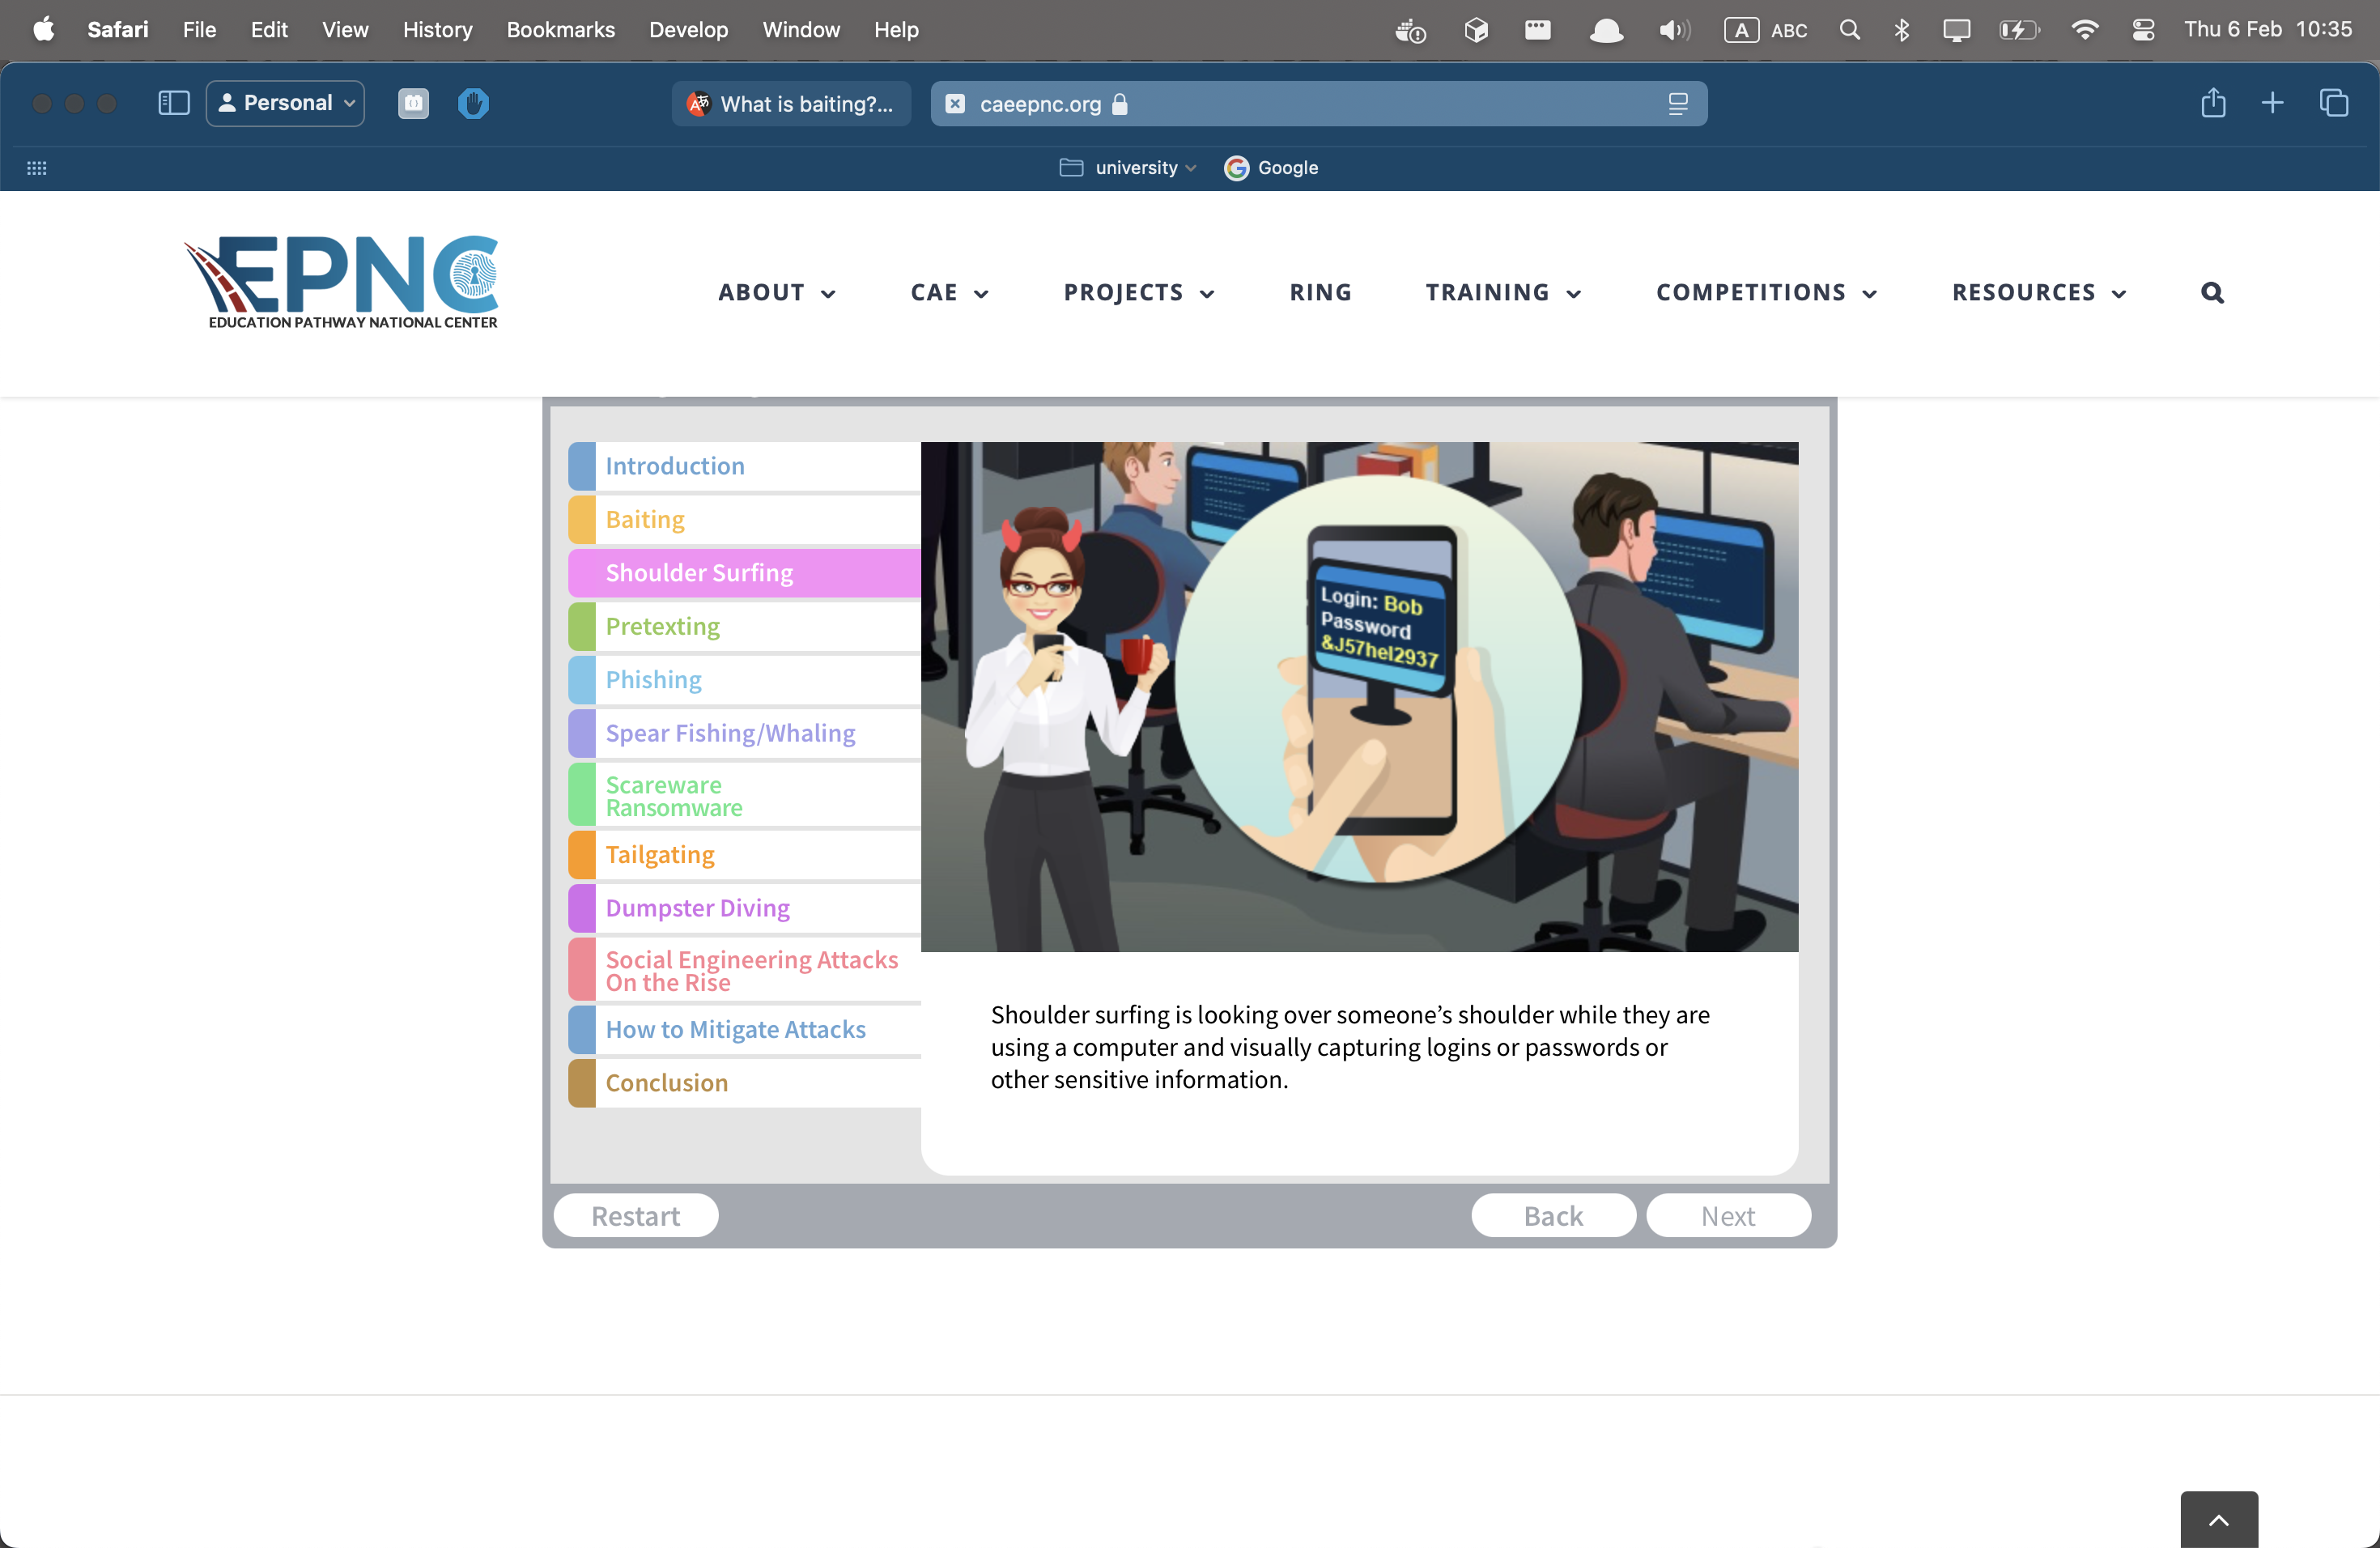
\includegraphics[width=1\textwidth]{2.png}

\newpage

\textbf{Question 3: } What is Pretexting? What type of information did the cybercriminal request? Would you fall victim? \\
\textbf{Answer: } Pretexting is a social engineering attack that uses deception to create a scenario to convince victims to divulge information they should not divulge. In the interactive game, cymbercriminal requested the name, title, office and employee badge number. And yes I fall victim. \\

\vspace{1\baselineskip}

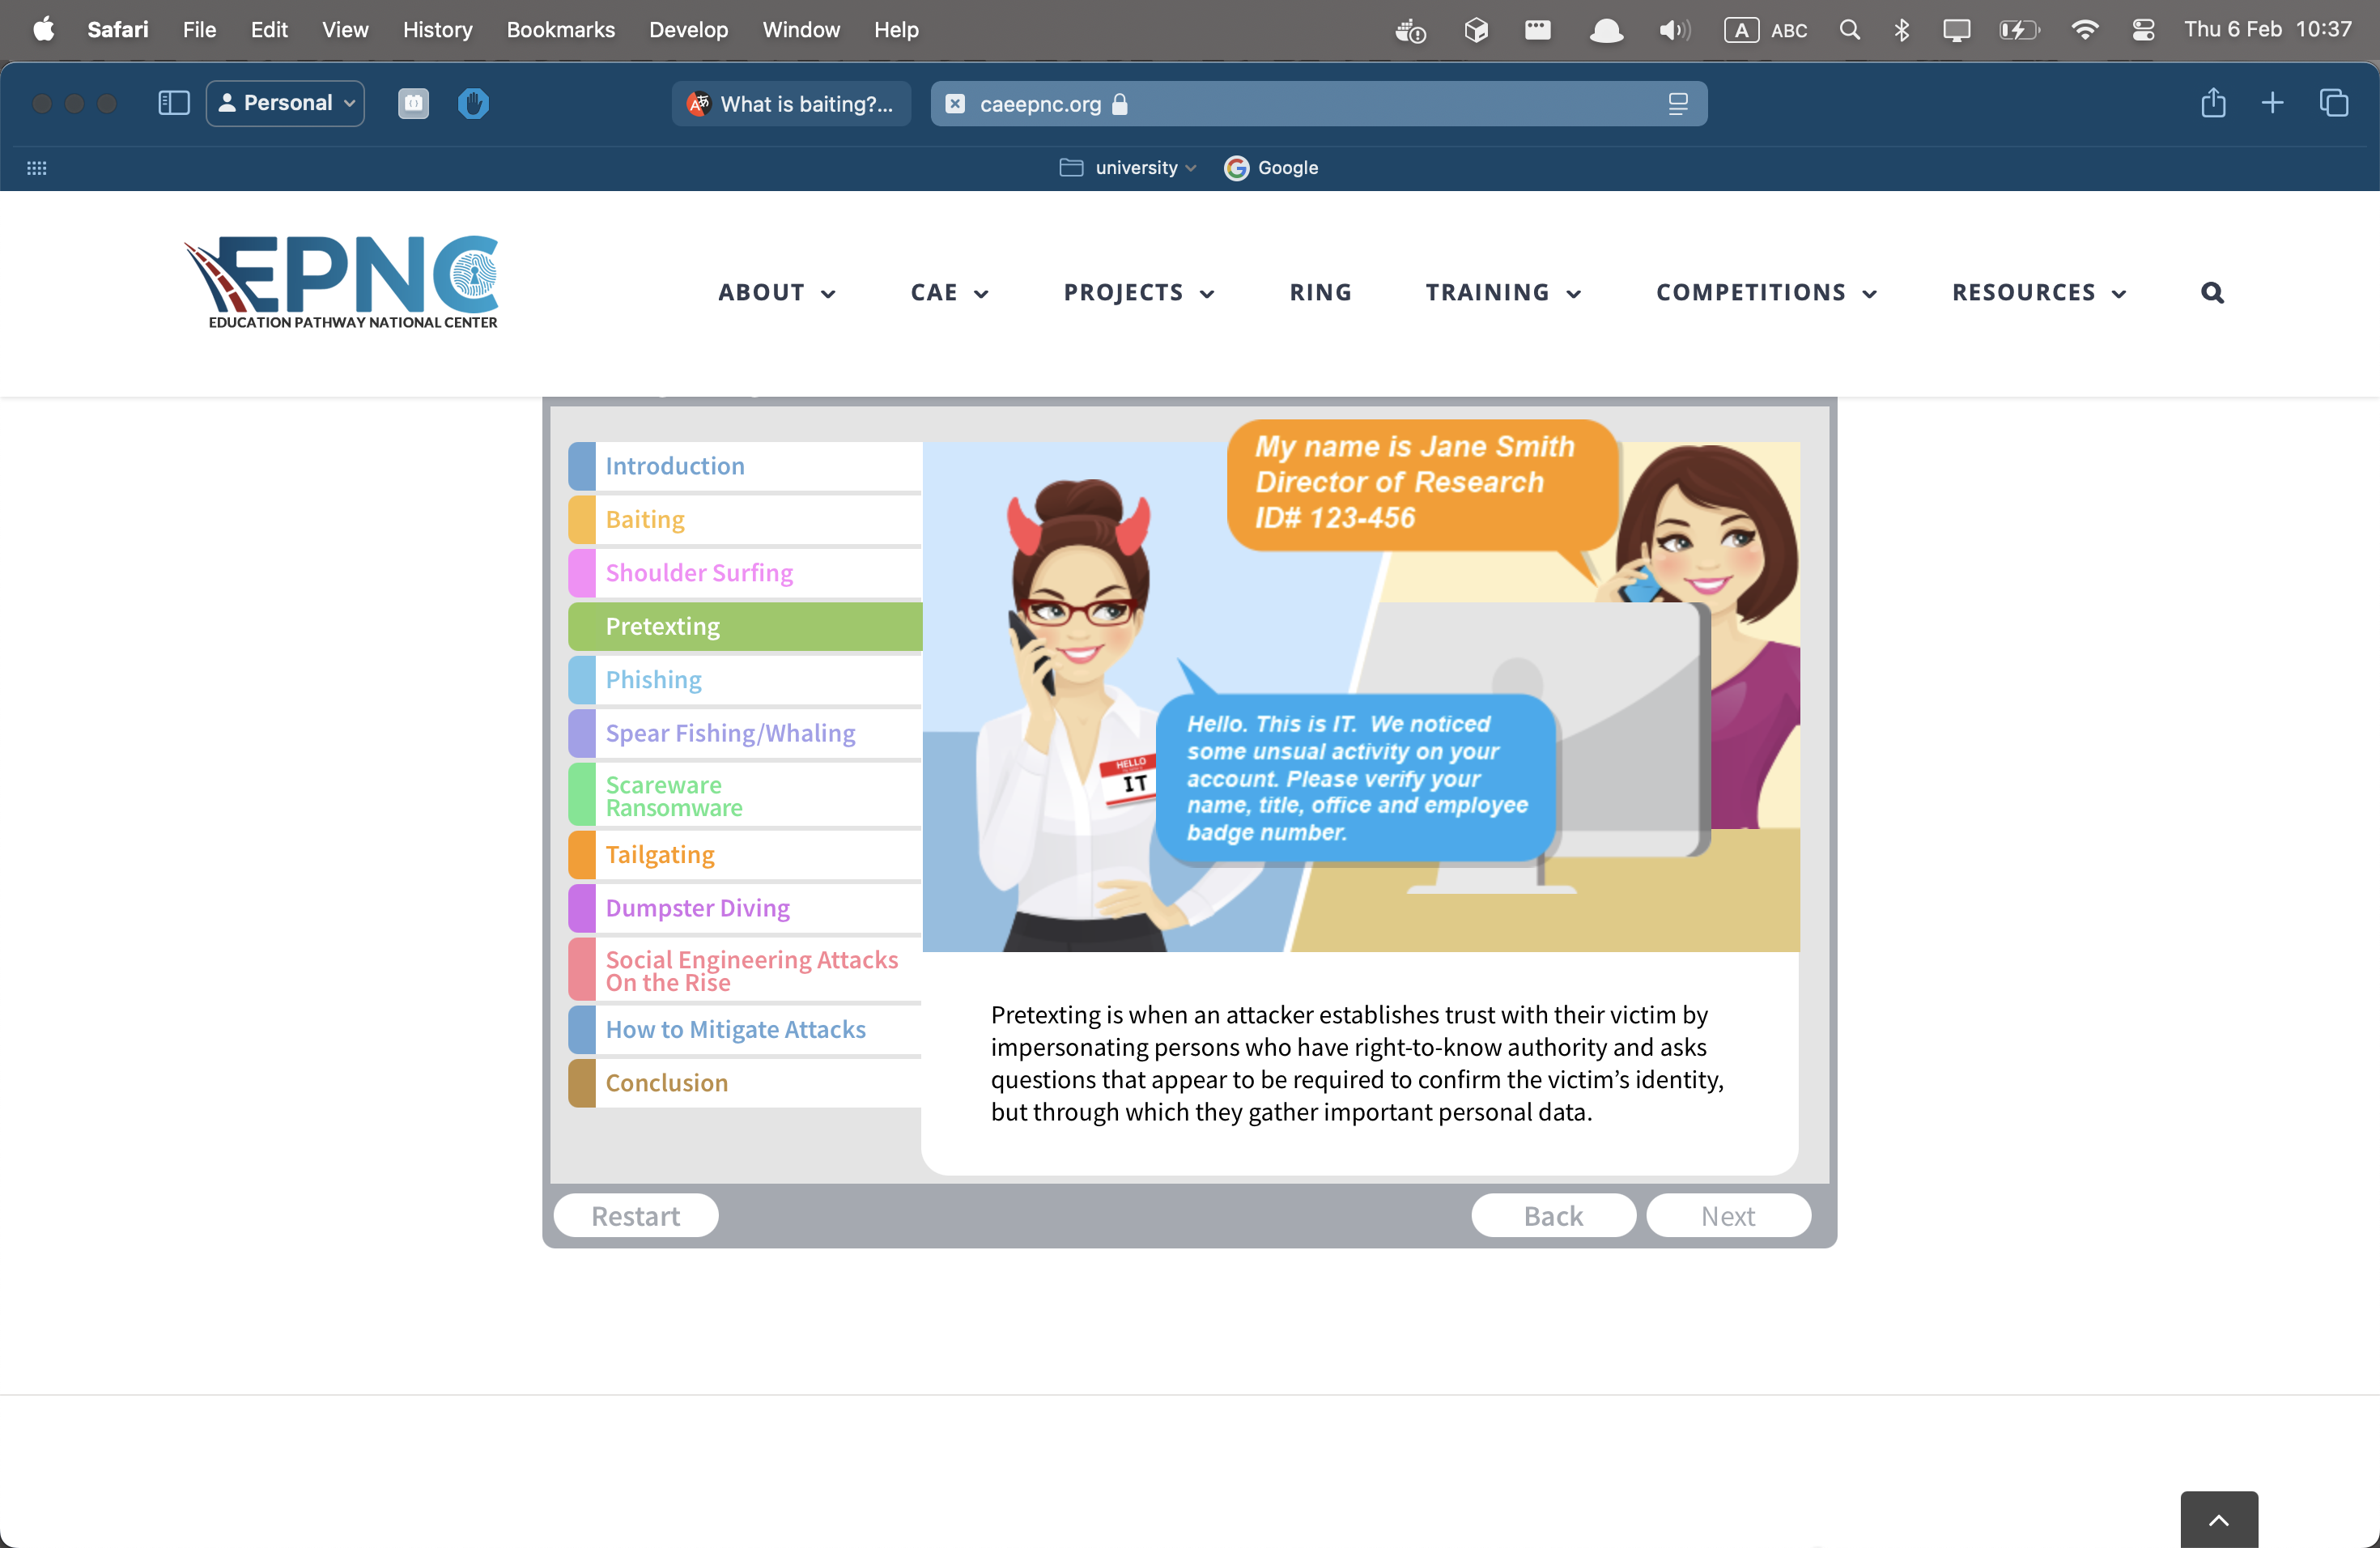
\includegraphics[width=1\textwidth]{3.png}

\newpage

\subsection*{Step 2: Explore Phishing, Spear Phishing, and Whaling}

\textbf{Question 1: } In this phishing example, what is the ploy the attacker uses to trick the victim to visit the trap website? What is the trap website used for? \\
\textbf{Answer: } The attacker pretended to be a trusted bank and asked to confirm whether he would withdraw money from the account, the victim fell for it and went to the phishing site and entered his secret data from the bank account. \\

\vspace{1\baselineskip}

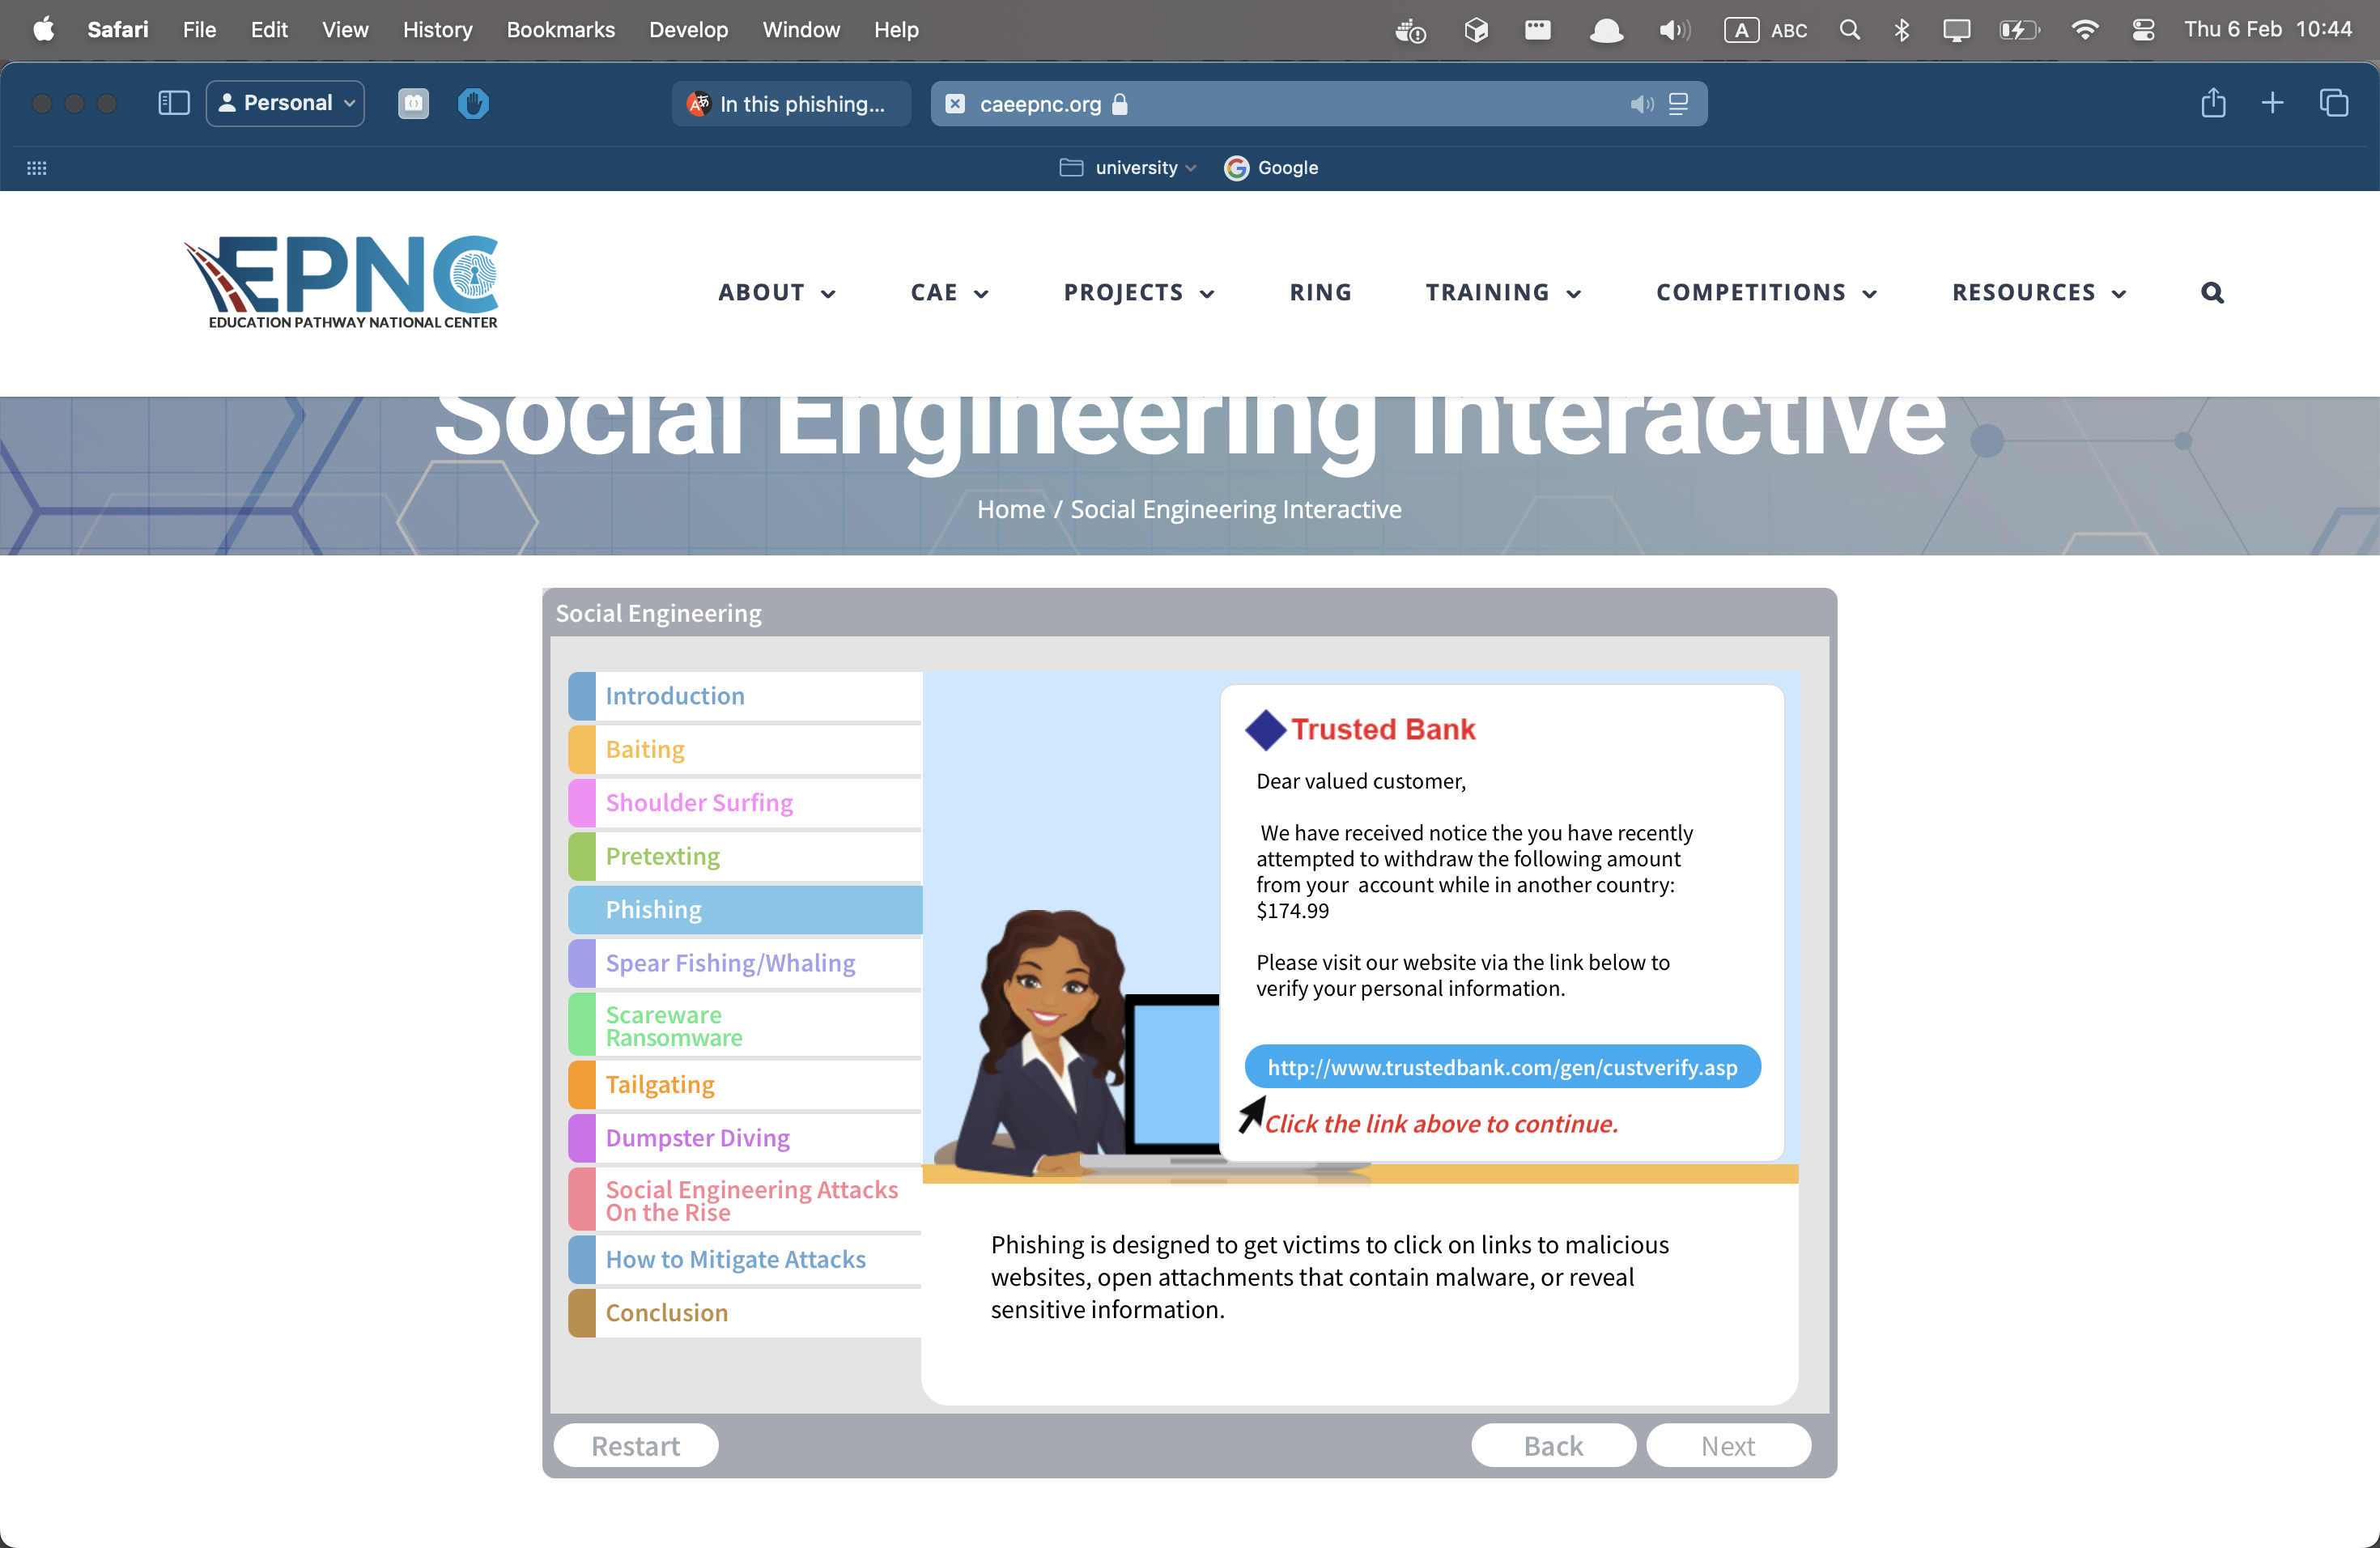
\includegraphics[width=1\textwidth]{4.png}

\vspace{1\baselineskip}

\textbf{Question 2: } What is the difference between phishing and spear phishing or whaling? \\
\textbf{Answer: } Phishing is a type of social engineering attack that targets a large number of people, while spear phishing is a more targeted version of phishing that targets specific individuals or enterprises. Whaling is a type of spear phishing that targets high-profile employees such as CEOs or CFOs. \\

\newpage

\subsection*{Step 3: Explore Scareware and Ransomware}

\textbf{Question 1: }What data does the attacker claim to have in this example? Would you fall for this deception? \\
\textbf{Answer: } Was claimed data about facebook login, credit bank account and email account. No i never fall for this deception. \\

\vspace{1\baselineskip}

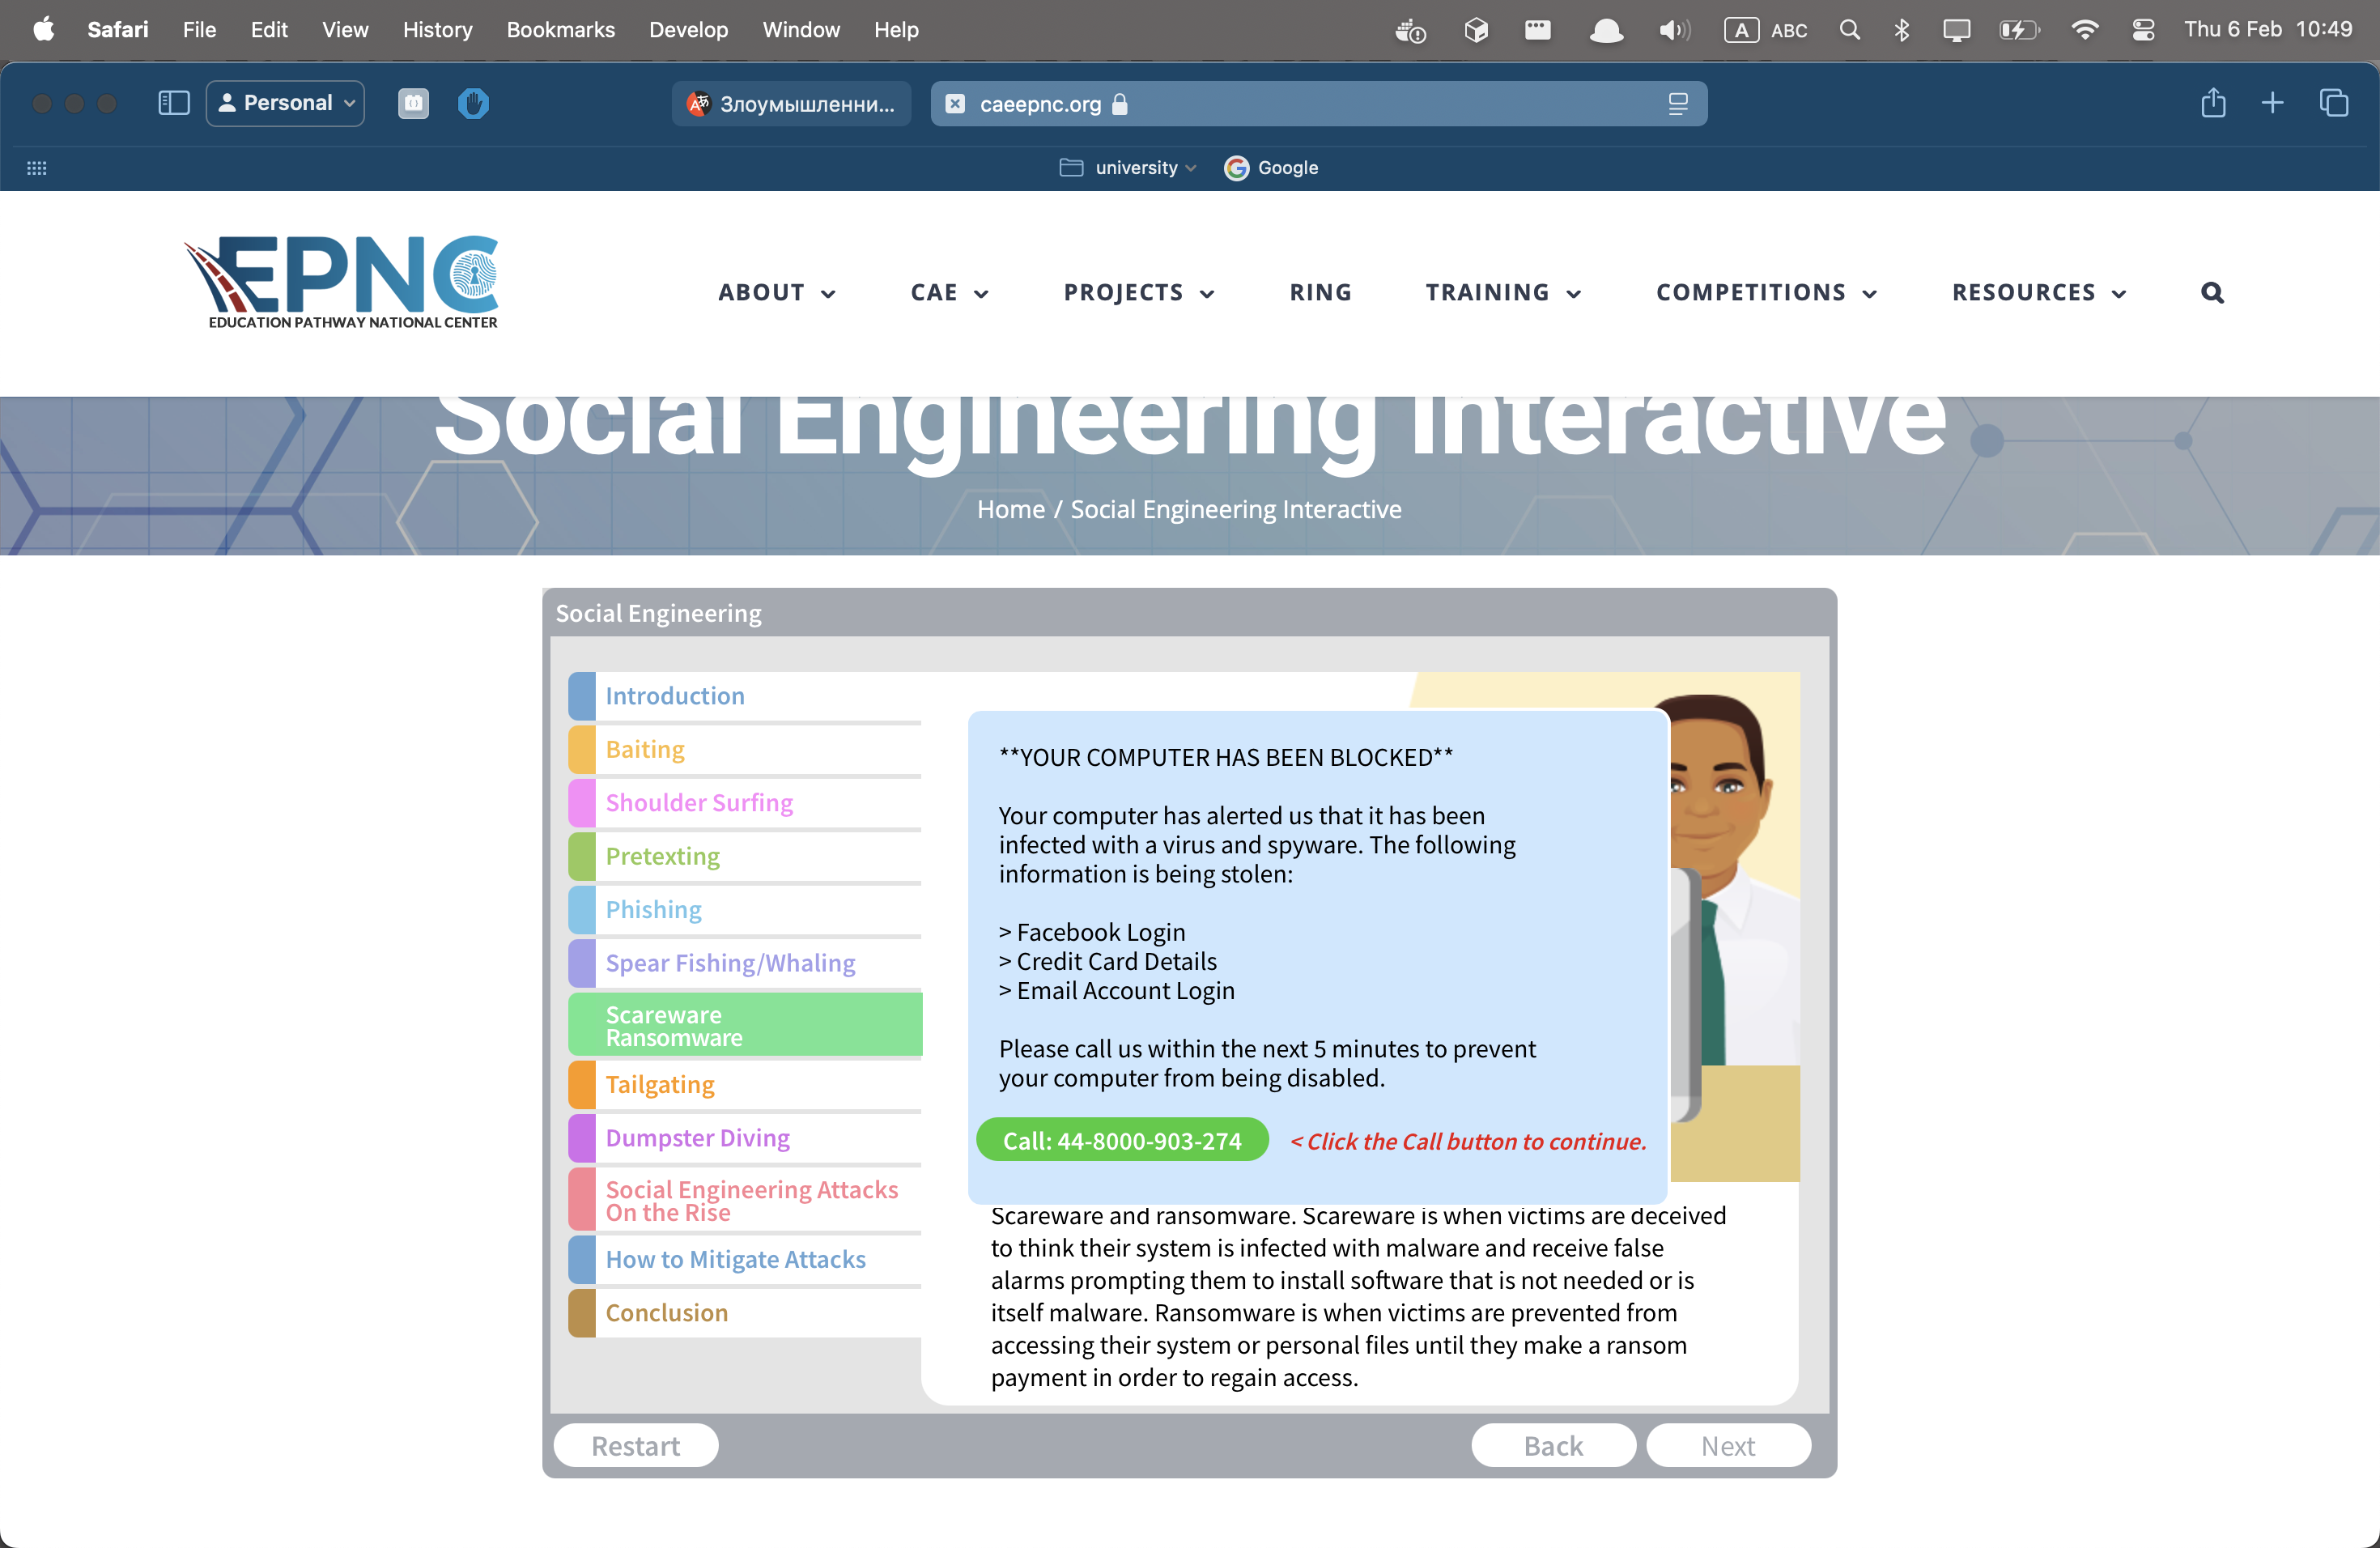
\includegraphics[width=1\textwidth]{5.png}

\newpage

\vspace{1\baselineskip}

\textbf{Question 2: } What is the attacker requesting the victim do to get the data back? \\
\textbf{Answer: } The attacker is requesting the victim to pay a ransom to get the data back. \\

\vspace{1\baselineskip}

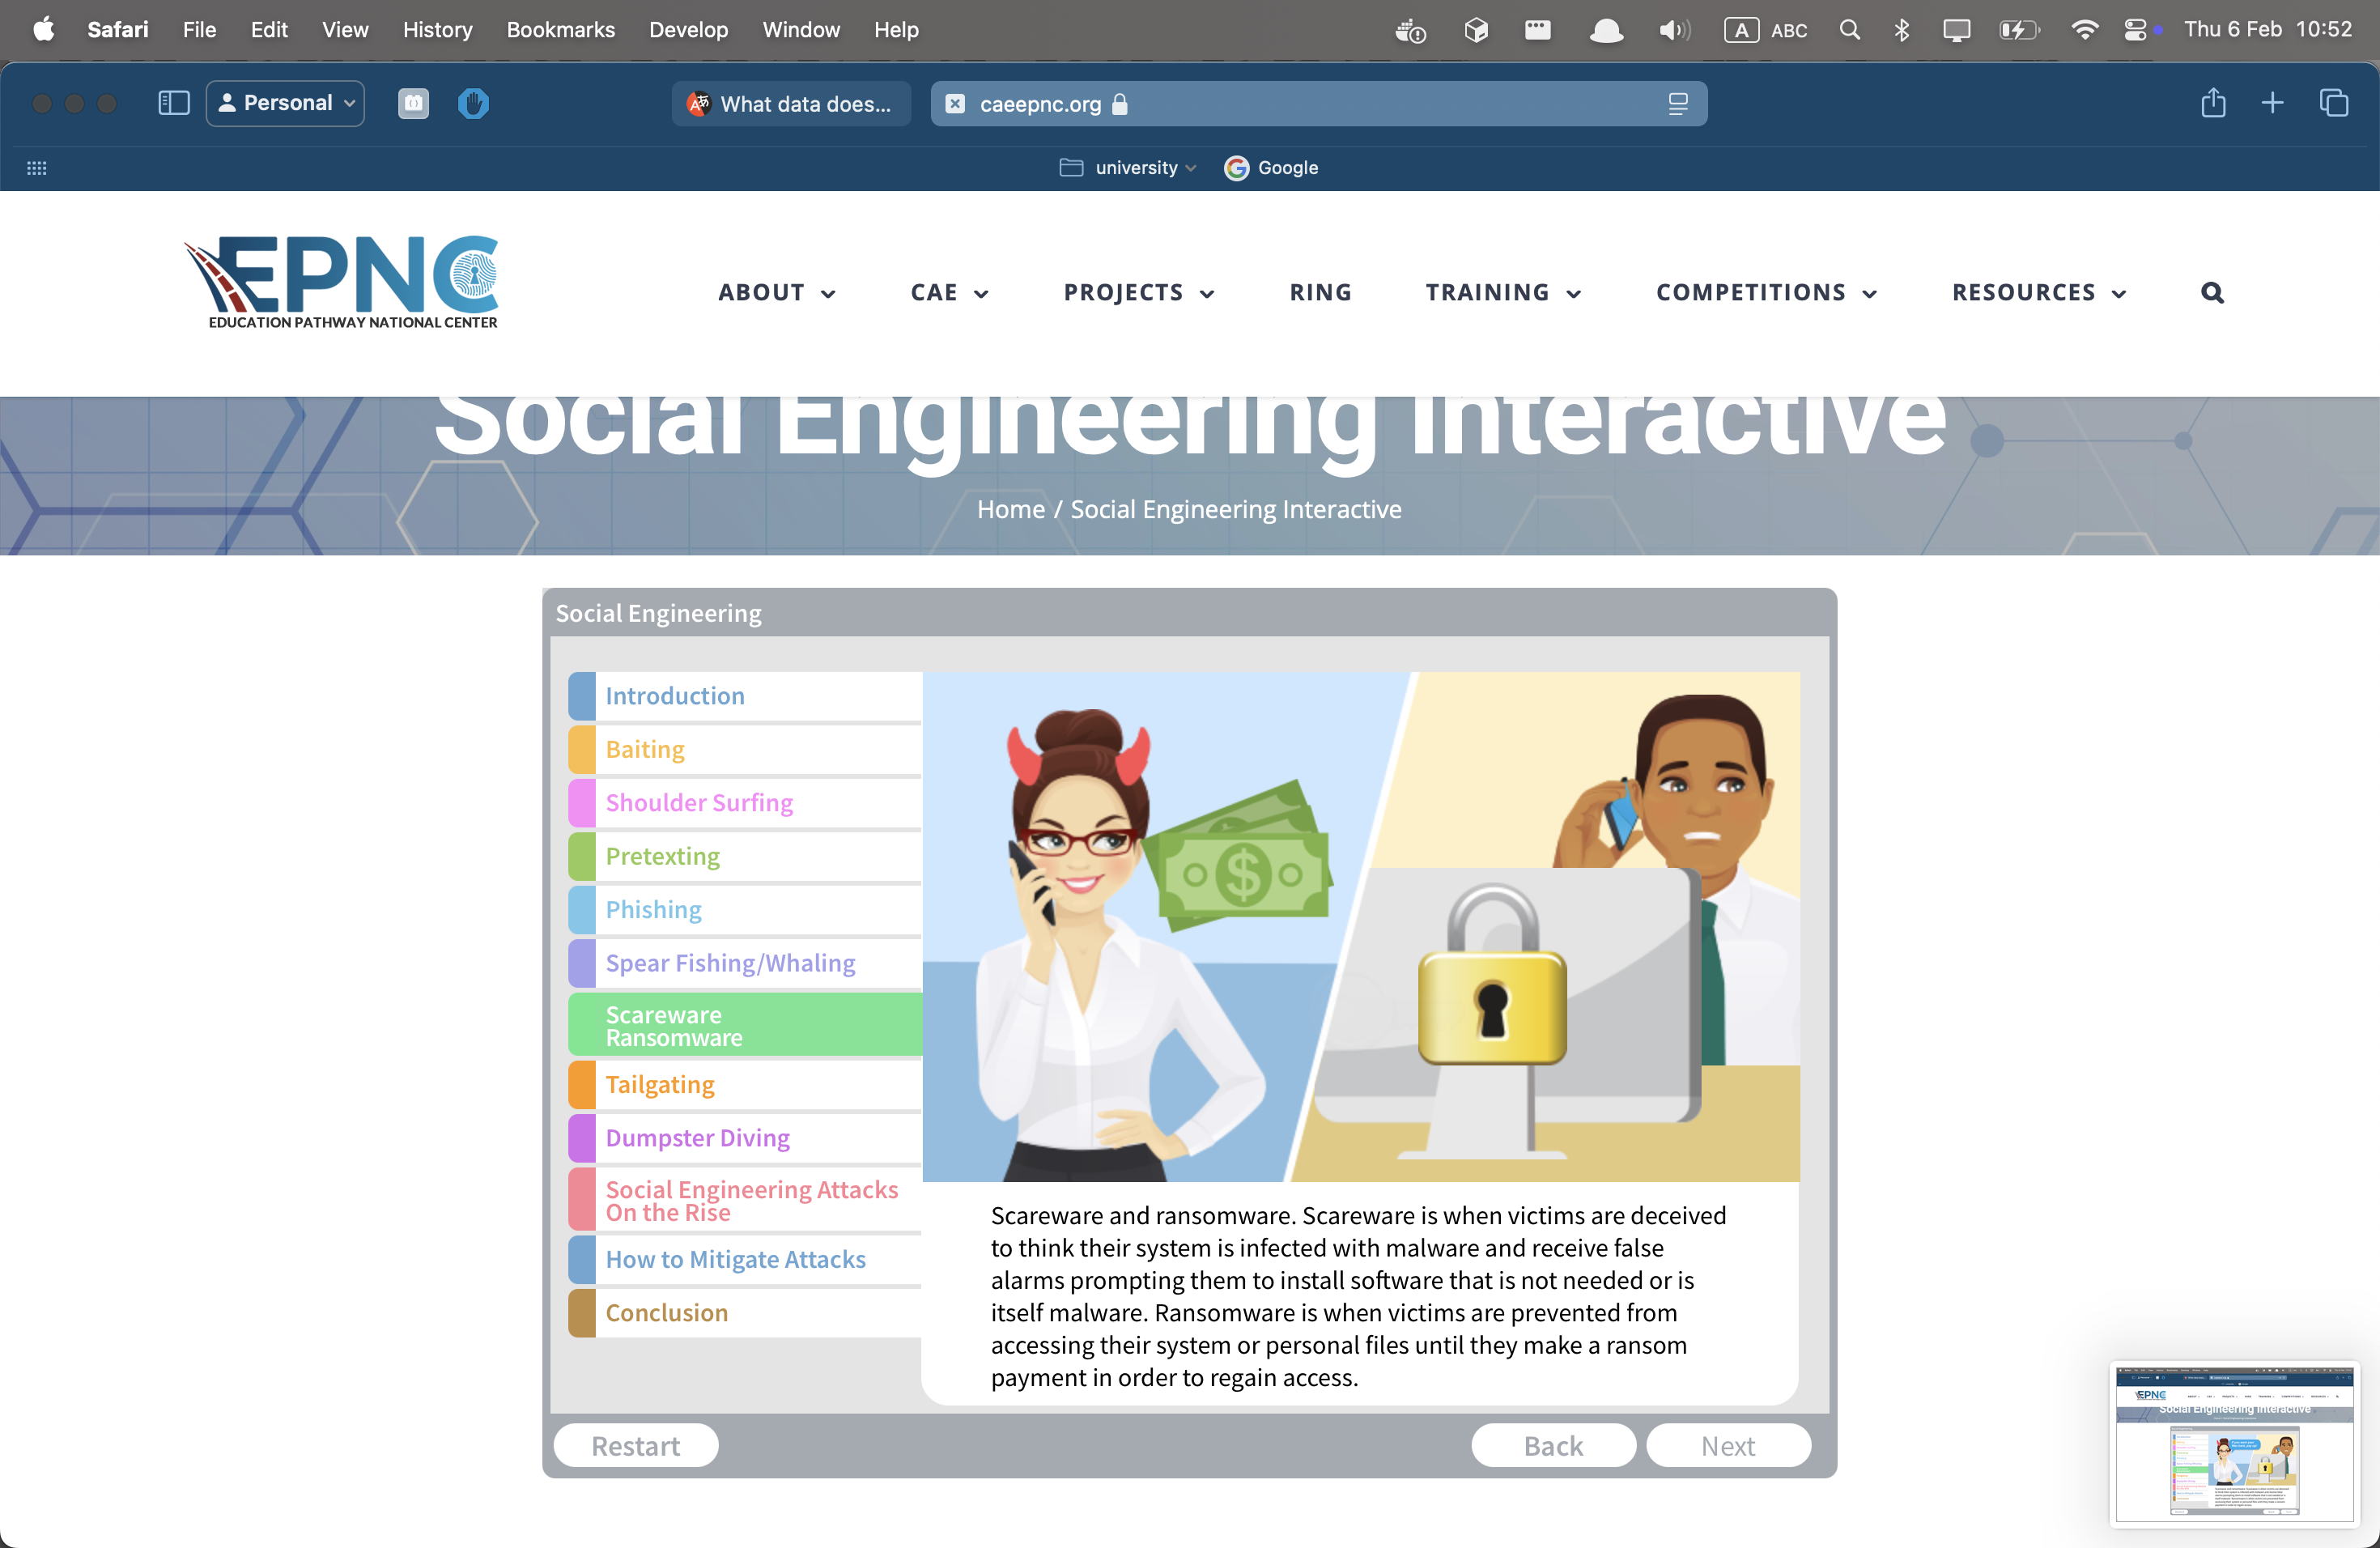
\includegraphics[width=1\textwidth]{6.png}

\vspace{1\baselineskip}

\textbf{Question 3: } What is tailgating? \\
\textbf{Answer: } Tailgating is a social engineering attack that tricks the victim into helping the attacker gain unauthorized access to the organization's physical facilities. \\

\vspace{1\baselineskip}

\textbf{Question 4: } Give three ways to prevent social engineering attacks? \\
\textbf{Answer: }
\begin{enumerate}
    \item Always verify the identity of the person requesting sensitive information, either through a phone call or in-person verification.
    \item Do not click on links or download attachments from unknown or suspicious emails.
    \item Regularly update and patch your software and systems to protect against known vulnerabilities.
\end{enumerate}


\end{document}